%\appendix
\begin{landscape}
\subsection{Software Sequence Diagram} \label{sec:appB}

\subsubsection{Air Sampling Control Object Sequence diagrams}
\begin{figure}[H]
    \centering
    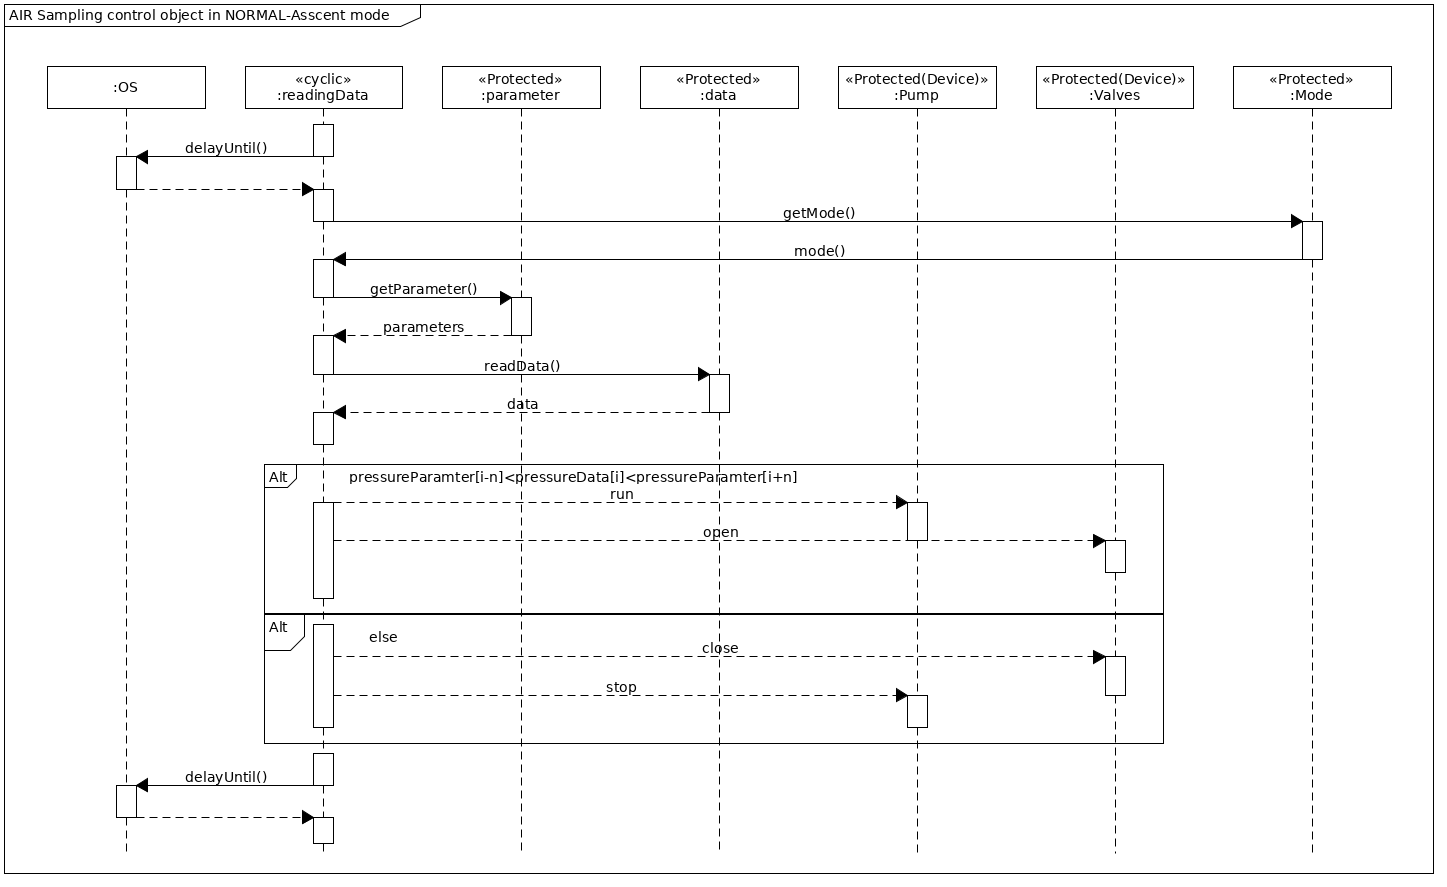
\includegraphics[height=0.75\textwidth]{appendix/img/ASC-seq-dia-v1-2-a.png}
    \caption{ASC Object in Normal Mode - Ascent.}
    \label{ASCa}
\end{figure}

\begin{figure}[H]
    \centering
    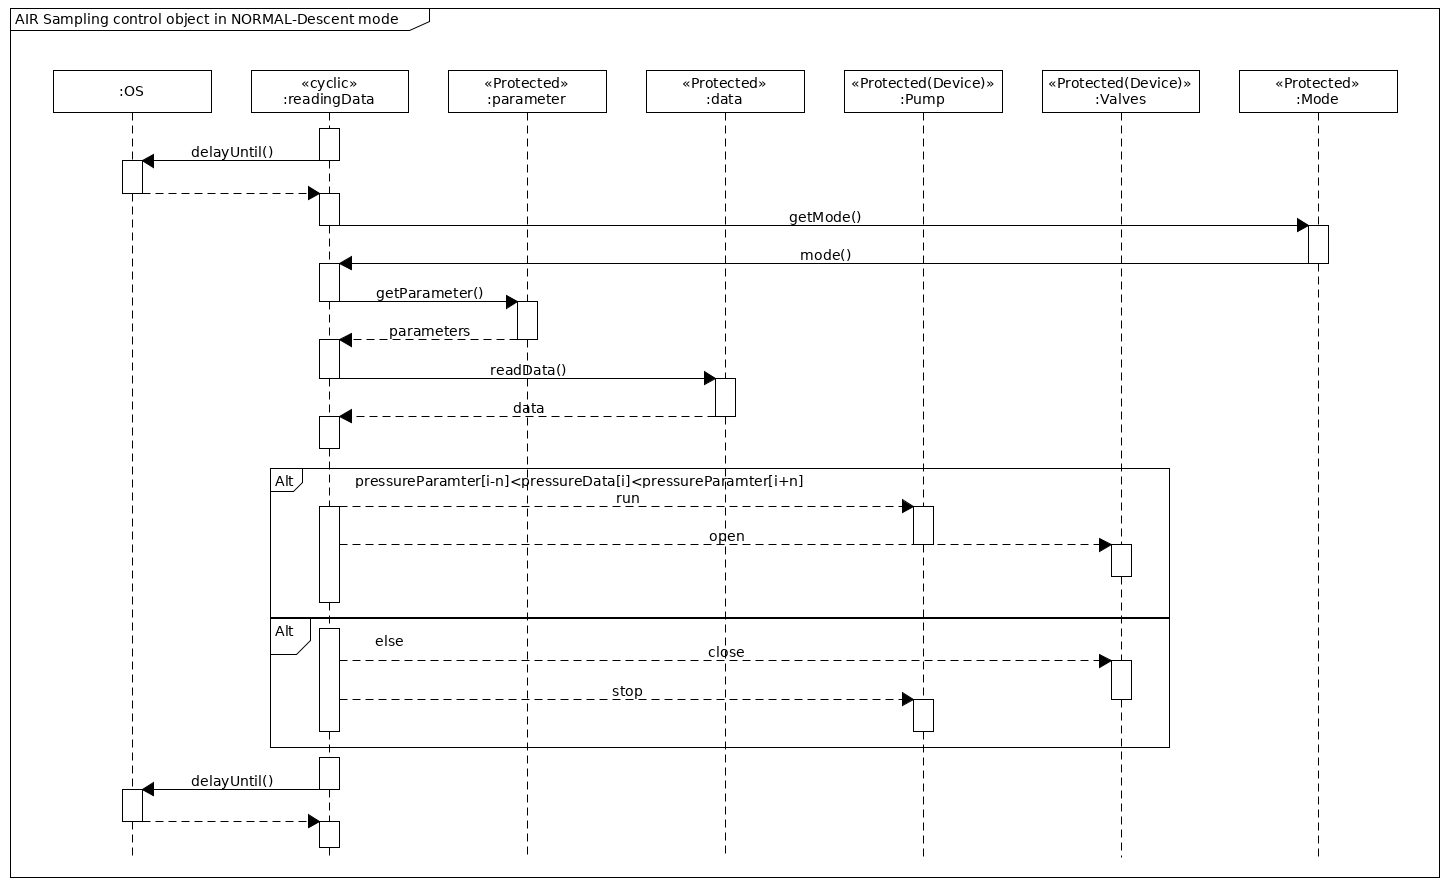
\includegraphics[height=0.9\textwidth]{appendix/img/ASC-seq-dia-v1-2-b.png}
    \caption{ASC Object in Normal Mode - Descent.}
    \label{ASCb}
\end{figure}
\begin{figure}[H]
    \centering
    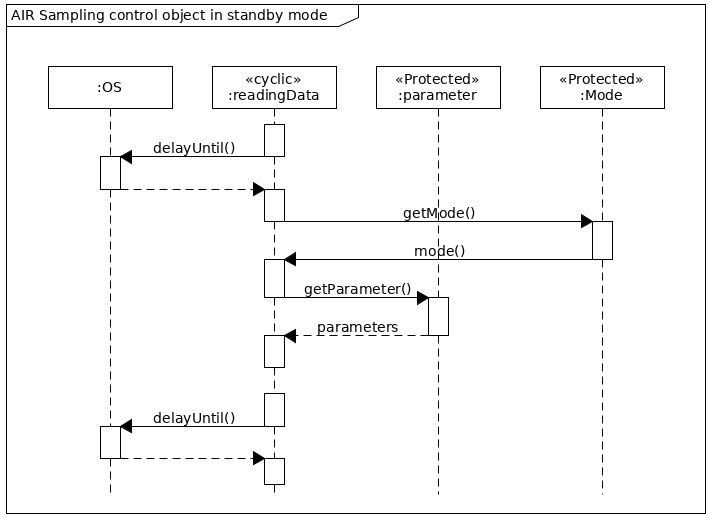
\includegraphics[height=0.9\textwidth]{appendix/img/ASC-seq-dia-v1-2-c.png}
    \caption{ASC Object in Standby Mode.}
    \label{ASCb}
\end{figure}
\subsection{Heating Object Sequence Diagrams}
\begin{figure}[H]
    \centering
    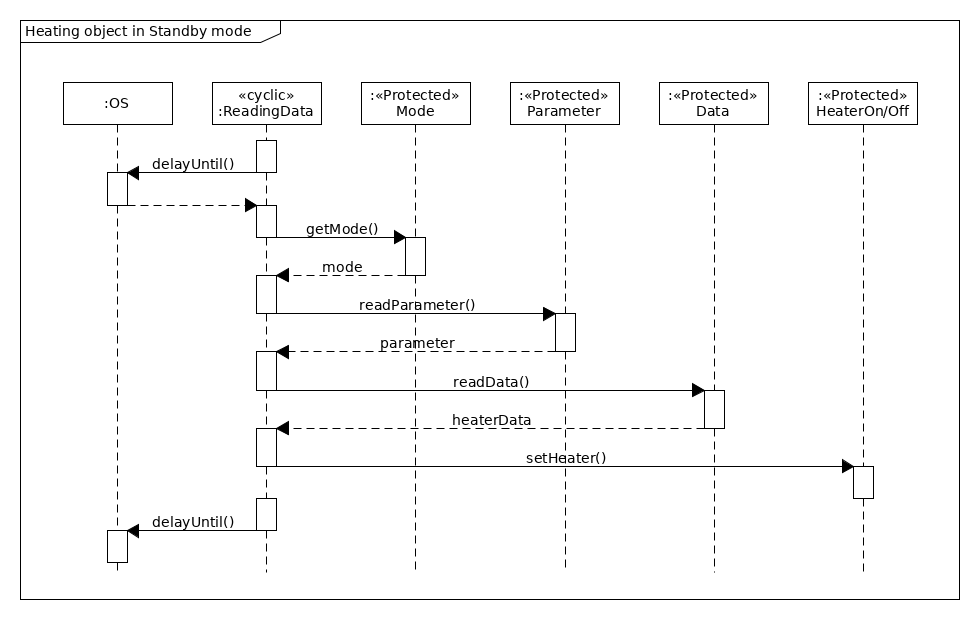
\includegraphics[height=0.8\textwidth]{appendix/img/heater-seq-dia-a.png}
    \caption{Heating Object in Standby Mode.}
    \label{heatera}
\end{figure}
\begin{figure}[H]
    \centering
    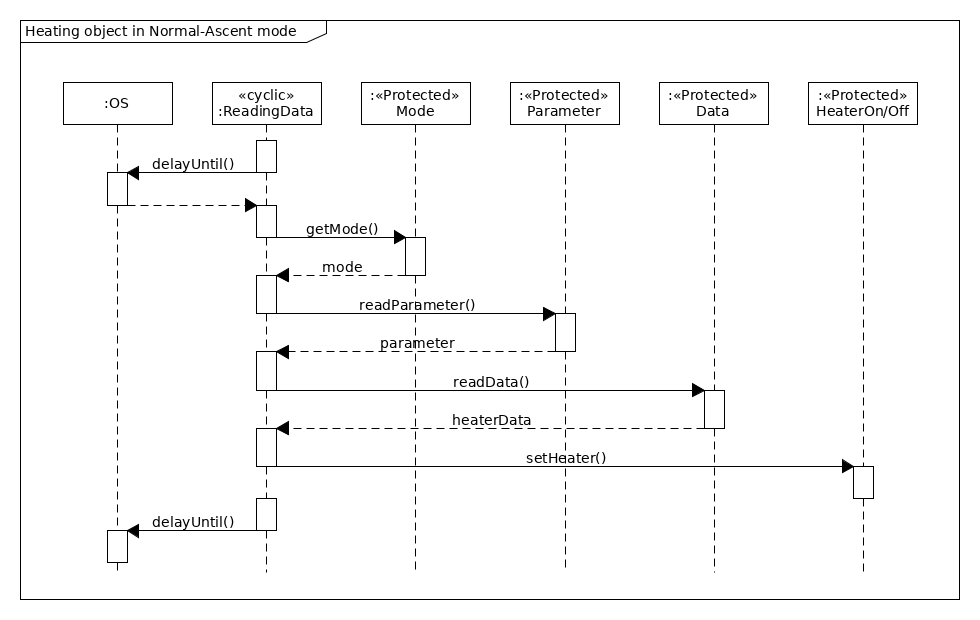
\includegraphics[height=0.9\textwidth]{appendix/img/heater-seq-dia-b.png}
    \caption{Heating Object in Normal Mode - Ascent.}
    \label{heaterb}
\end{figure}
\begin{figure}[H]
    \centering
    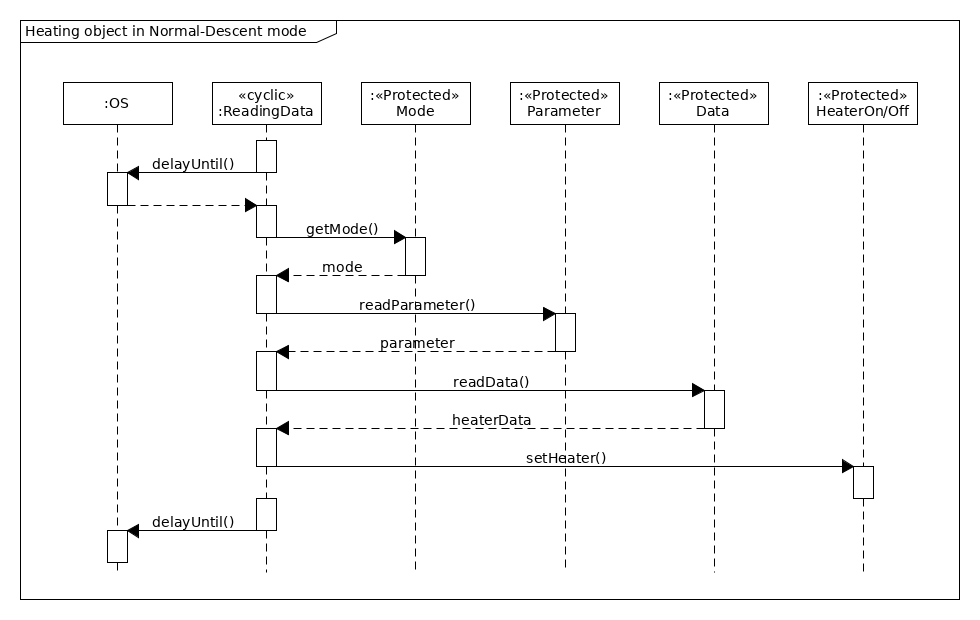
\includegraphics[height=0.9\textwidth]{appendix/img/heater-seq-dia-c.png}
    \caption{Heating Object in Normal Mode - Descent.}
    \label{heaterc}
\end{figure}
\subsection{Sensor Object Sequence Diagrams}
\begin{figure}[H]
    \centering
    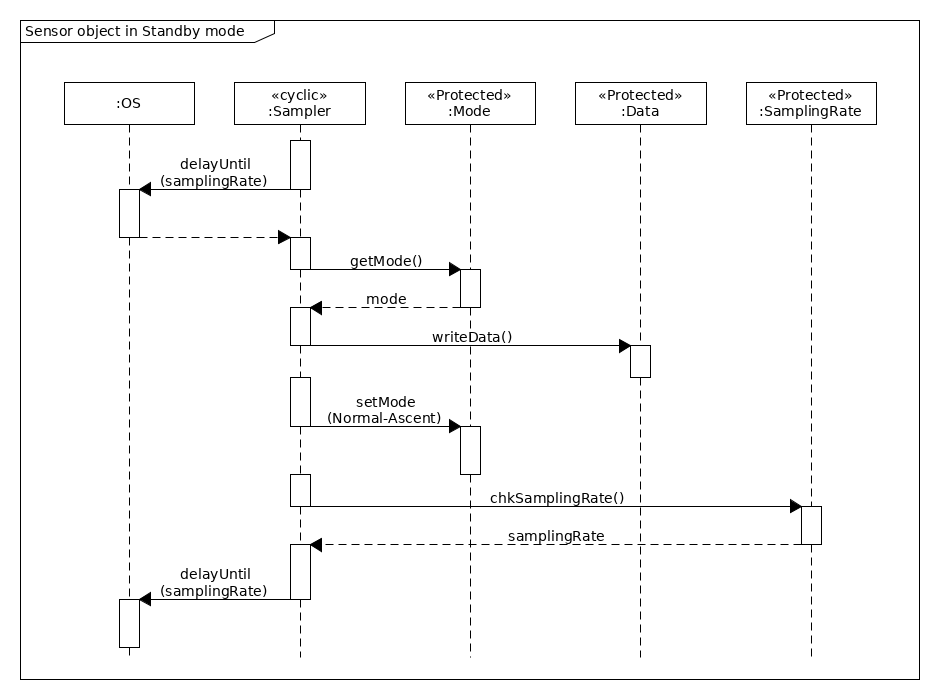
\includegraphics[height=0.8\textwidth]{appendix/img/sensor-seq-dia-a.png}
    \caption{Sensor Object in Standby Mode.}
    \label{sensora}
\end{figure}
\begin{figure}[H]
    \centering
    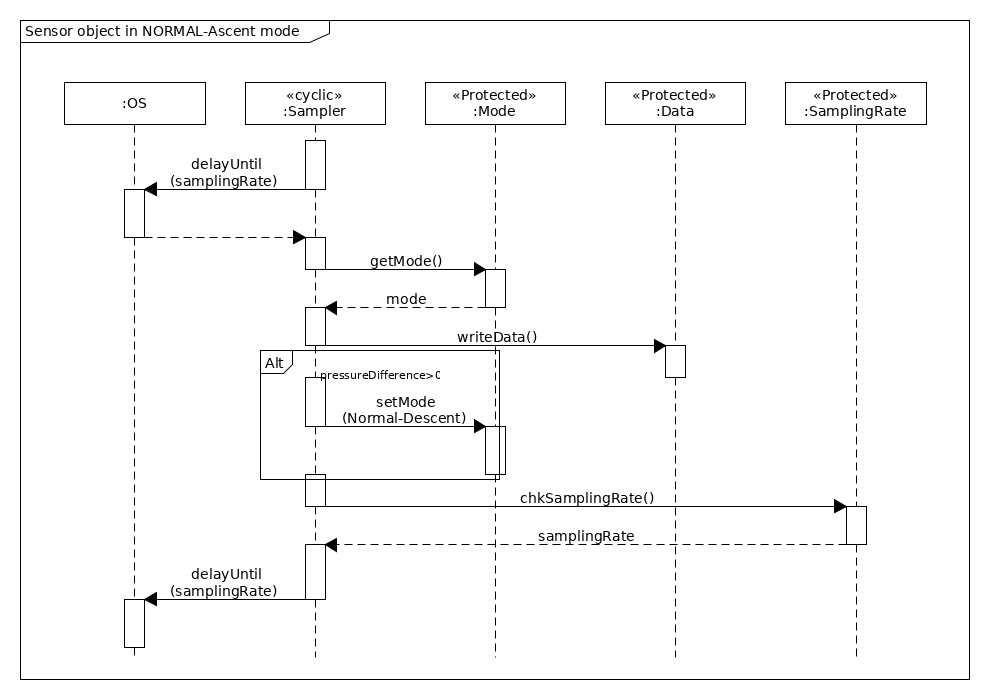
\includegraphics[height=0.9\textwidth]{appendix/img/sensor-seq-dia-b.png}
    \caption{Sensor Object in Normal - Ascent Mode.}
    \label{sensorb}
\end{figure}
\begin{figure}[H]
    \centering
    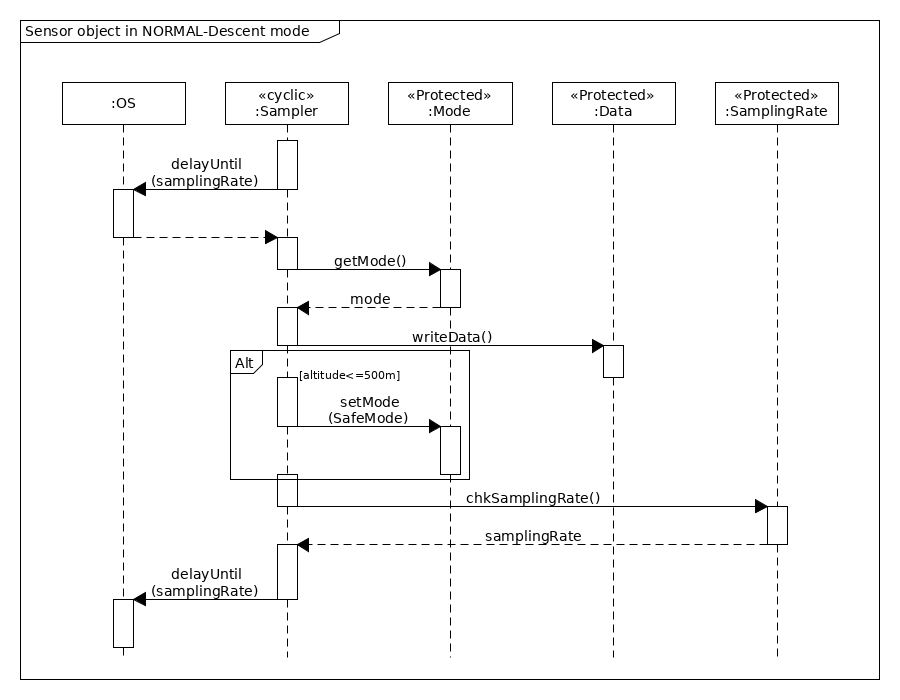
\includegraphics[height=0.9\textwidth]{appendix/img/sensor-dia-seq-c.png}
    \caption{Sensor Object in Normal - Descent Mode.}
    \label{sensorc}
\end{figure}
\end{landscape}